\newpage
\section{AI  System Solution}
The main application continuously analyzes the driver’s state, focusing on age and gender prediction, drowsiness detection, and distraction detection using artificial intelligence methods. The system captures and processes video data in real-time by utilizing infrared (IR) or RGB images.\\

Our approach simplifies the process by using a deep learning model for face detection and classical machine learning and image processing techniques for further analysis. After detecting faces, the system extracts facial landmarks. These landmarks are then used to estimate head pose, monitor eye and mouth aspect ratios, and track eye gaze direction to identify signs of drowsiness and distraction.\\

This method is computationally efficient, enabling real-time performance, and adaptable to different lighting conditions. 

\subsection{ Face Feature Extraction}

In driver monitoring systems, the extraction of facial features plays a critical role in ensuring accurate and reliable detection of driver states such as drowsiness and distraction. This process involves several key steps, each contributing to the system's overall effectiveness. The system's design is depicted in Fig. 1. The DMS employs a camera (imager) as the input image source, and the captured image is used for face detection followed by facial landmarks estimation. These extracted facial landmarks serve as crucial features for estimating head pose and identifying instances of closed eyes and yawning, indicative of drowsy driving.

\subsubsection{Face Detection Using YOLOv8n}

The first step in facial feature extraction involves detecting the driver's face using YOLOv8, or You Only Look Once version 8. YOLOv8 is a 1-stage detection algorithm, similar to the SSD detector, offering both satisfactory performance and fast processing speed, specifically the nano version implemented by Ultralytics. As shown in Fig. 2, the nano version is chosen for its efficient use of computational resources without compromising on detection accuracy, making it ideal for real-time applications in resource-constrained environments. \\

Trained on the comprehensive WIDERFACE dataset. The WIDERFACE dataset is a large and diverse collection of over 32,000 images with nearly 400,000 labeled faces, designed to cover a wide range of challenging real-world scenarios for robust face detection.\\

The model generates bounding boxes that precisely outline each detected face, defined by coordinates for the top-left corner and dimensions. These bounding boxes are accompanied by confidence scores, quantifying the model's certainty that the box contains a face. \\

PyTorch was selected for training YOLO over TensorFlow for deployment in C++ environments and its capability to load models directly into memory, resulting in faster inference times crucial for real-time applications. PyTorch's support for seamless deployment across GPUs, CPUs, and custom accelerators ensures scalability and performance optimization. Additionally, its superior support for multithreading enhances efficiency in handling concurrent tasks, making it suitable for high-throughput applications.\\

\subsubsection{ Facial Landmarks Extraction}

Facial landmark extraction has made significant strides in recent years, with deep learning techniques like Openface and Retinaface at the forefront. However, in our DMS, the high computational costs associated with face detection using deep learning present a challenge. To mitigate this, we have chosen Kazemi's fast facial landmark extraction algorithm, which has been integrated into the Digital Library (Dlib) library. Kazemi’s algorithm, based on random forests, provides an excellent balance of speed and performance, making it suitable for the DMS, which needs to function efficiently in an embedded environment rather than a desktop setup.\\

Dlib's first step is face detection, then applying facial landmark extraction built on Kazemi's algorithm's principles. Dlib includes two face detection methods:
\begin{enumerate}
    \item HOG + Linear SVM Face Detector: \\
    This method accessible via dlib.get\_frontal\_face\_detector(), is known for its accuracy and computational efficiency.
    \item Max-Margin (MMOD) CNN Face Detector: \\
    This method is highly accurate and robust, capable of detecting faces under varying viewing angles, lighting conditions, and occlusion.
\end{enumerate}

For our system, we replace the HOG + Linear SVM face detection method with the YOLOv8 face detection model. YOLOv8 provides more accurate and faster face detection, which is crucial for the real-time requirements of our DMS. By leveraging the precise bounding boxes generated by YOLOv8, we can then feed these into Dlib for accurate facial landmarks. This is crucial for analyzing the driver's state, and detailed explanations of their use will be provided in subsequent sections.\\

We use the shape\_predictor\_68\_face\_landmarks\_GTX.dat.bz2 model, a highly optimized and accurate facial landmark detector. This model is trained on the ibug 300-W dataset, a comprehensive benchmark dataset containing a variety of images with annotated facial landmarks. The GTX version of the model utilizes advanced training strategies to enhance performance and accuracy, including data augmentation, robust optimization techniques, and meticulous fine-tuning to ensure the model can accurately predict 68 key facial landmarks under diverse conditions.\\

The output of this stage is the key 68 landmarks, which are then fed into other algorithms for further analysis. This integration ensures that our DMS can reliably monitor the driver states.

\subsubsection{Age and Gender Estimation}

In the context of diver monitoring systems, estimating the age and gender of divers is crucial for several reasons:

\begin{enumerate}
    \item \textbf{Safety Protocols:} Different age groups and genders may have varying physiological responses to underwater conditions. Understanding these differences can help tailor safety protocols to ensure the well-being of all divers.
\item \textbf{Personalized Experiences: }Personalized recommendations and experiences can enhance a diver's overall satisfaction. For instance, training programs can be customized based on the age and gender of the divers.
\item \textbf{Statistical Analysis:} Collecting demographic data allows for detailed analysis of diving patterns and trends, aiding in the development of targeted marketing strategies and improvement of services.
\end{enumerate}

\textbf{Models Provided by Dlib and Cydral Technology}\\
The pre-trained models for age and gender estimation used in this system are provided by Dlib and are available for free under the Creative Commons Zero v1.0 Universal license by Cydral Technology. These models offer robust performance due to their training on large, private datasets and their sophisticated architectures.\\

\textbf{Gender Classifier: "dnn\_gender\_classifier\_v1.dat.bz2"}\\
This gender classifier model was trained on approximately 200,000 face images. The training followed the architecture and settings outlined in the paper "Minimalistic CNN-based ensemble model for gender prediction from face images." Key features include:
\begin{itemize}
    \item \textbf{CNN Ensemble Model:} The use of a minimalistic CNN ensemble approach helps improve classification accuracy by leveraging multiple CNNs.
\item \textbf{Private Dataset:} The extensive dataset ensures that the model generalizes well to diverse real-world scenarios.
\end{itemize}











\subsection{Eye Closure Detection}

In our previous discussions, we explored how to apply facial landmark detection to identify key regions of the face, such as the eyes, eyebrows, nose, ears, and mouth. This capability allows us to extract specific facial structures by referencing the indexes of particular face parts.

\begin{figure}[H]
    \centering
    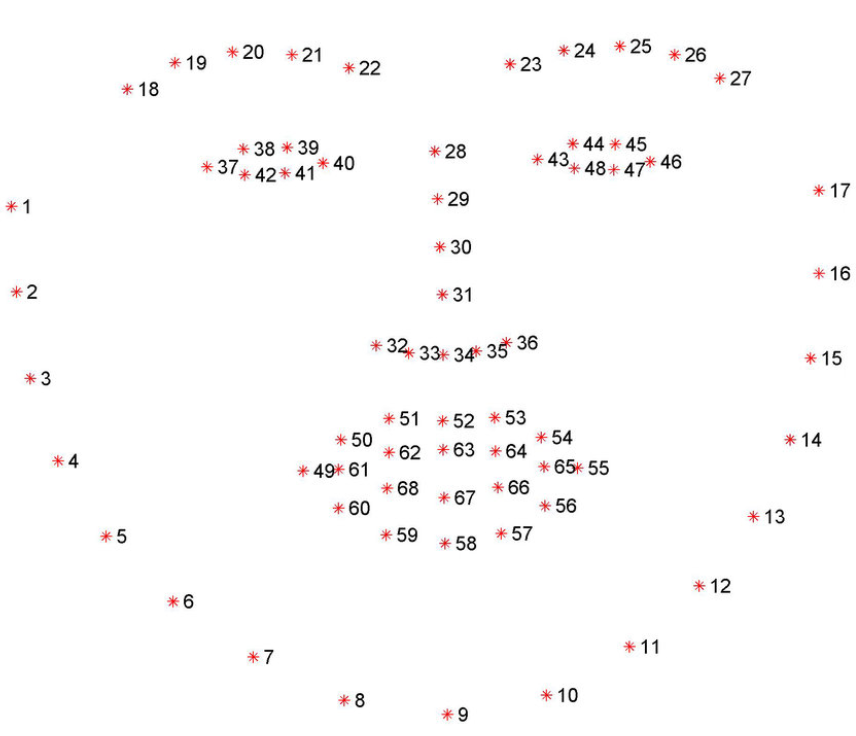
\includegraphics[width=0.7\textwidth]{Images/1_AI/68_face_landmarks.png}
    \caption{Applying facial landmarks to localize various regions of the face, including eyes, eyebrows, nose, mouth, and jawline.}
    \label{fig:68_face_landmarks}
\end{figure}

For the purpose of blink detection, we focus on two sets of facial structures: the eyes.

Each eye is represented by six (x, y)-coordinates, starting at the left corner of the eye (as if you were looking at the person) and moving clockwise around the rest of the region.

\begin{figure}[H]
    \centering
    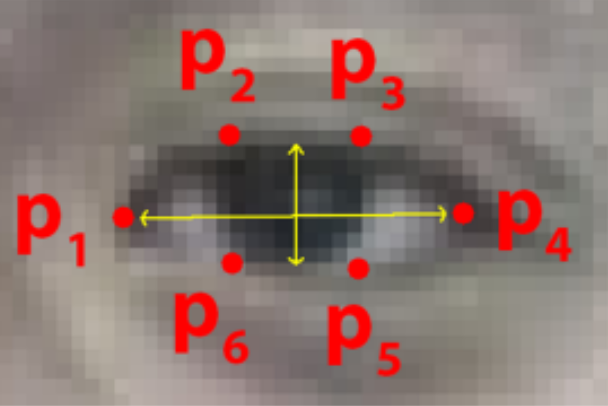
\includegraphics[width=0.5\textwidth]{Images/1_AI/6points_open_eye.png}
    \caption{The six facial landmarks associated with the eye.}
    \label{fig:6points_open_eye}
\end{figure}

Building on the work by Soukupová and Čech in their 2016 paper, *Real-Time Eye Blink Detection using Facial Landmarks*, we derive an equation reflecting this relationship, known as the eye aspect ratio (EAR):

\begin{equation}
\text{EAR} = \frac{\|p_2 - p_6\| + \|p_3 - p_5\|}{2 \|p_1 - p_4\|}
\end{equation}

where \( p_1, \ldots, p_6 \) are 2D facial landmark locations. The numerator calculates the distance between the vertical eye landmarks, while the denominator computes the distance between horizontal eye landmarks, with appropriate weighting since there is only one set of horizontal points but two sets of vertical points.

The eye aspect ratio remains approximately constant when the eye is open but rapidly decreases to zero when a blink occurs. This simple equation enables us to detect blinks by relying on the ratio of eye landmark distances, bypassing the need for complex image processing techniques.

Consider the following figures:

\begin{figure}[H]
    \centering
    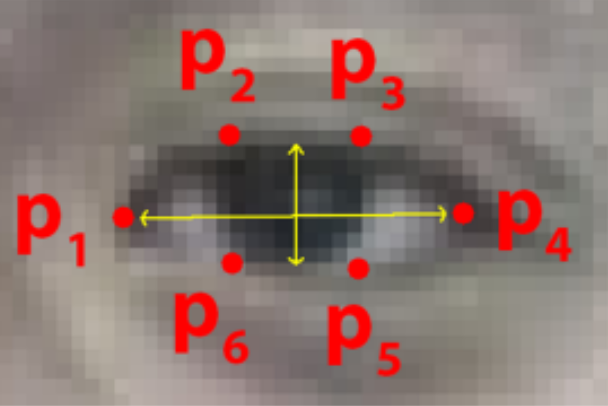
\includegraphics[width=0.8\textwidth]{Images/1_AI/6points_open_eye.png}
    \caption{Eye landmarks when the eye is open.}
    \label{fig:6points_open_eye}
\end{figure}

\begin{figure}[H]
    \centering
    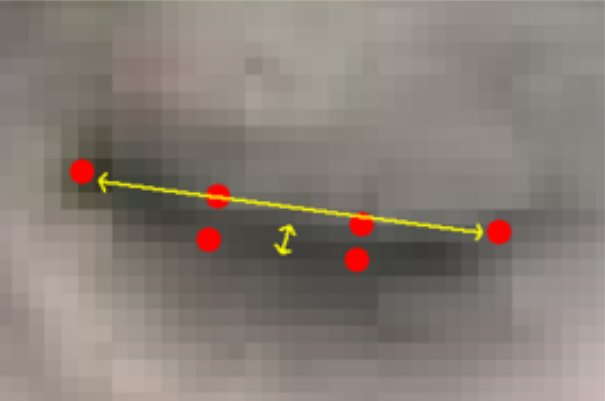
\includegraphics[width=0.8\textwidth]{Images/1_AI/6points_closed_eye.png}
    \caption{Eye landmarks when the eye is closed.}
    \label{fig:6points_closed_eye}
\end{figure}

\begin{figure}[H]
    \centering
    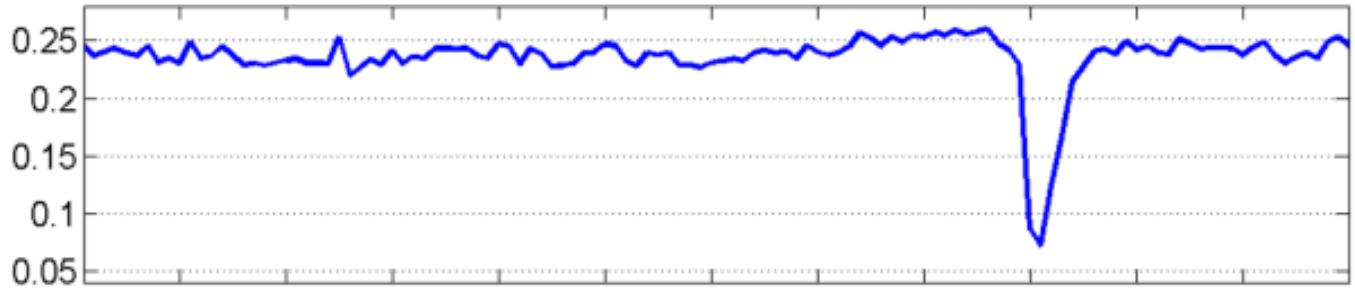
\includegraphics[width=0.8\textwidth]{Images/1_AI/ear_over_time.png}
    \caption{Plotting the eye aspect ratio over time. The dip in the eye aspect ratio indicates a blink.}
    \label{fig:ear_over_time}
\end{figure}

In Figure \ref{fig:Eye_landmarks_open}, the eye is fully open, and the eye aspect ratio is relatively large and constant. When the person blinks (Figure \ref{fig:Eye_landmarks_closed}), the eye aspect ratio drops significantly, approaching zero.

To determine whether the eye is open or closed based on the Eye Aspect Ratio (EAR), a threshold value is crucial. Typically, the eye is classified as closed when the EAR drops below a specified threshold, such as the commonly recommended value of around \textcolor{red}{0.25}. This value ensures accurate detection of blinks and prolonged eye closures, critical for evaluating driver alertness in driver monitoring systems. Adjusting the threshold to approximately \textcolor{red}{0.25} enhances performance under different lighting conditions and facial orientations.

Figure \ref{fig:ear_over_time} plots the eye aspect ratio over time for a video clip. As observed, the eye aspect ratio remains constant, then drops near zero, and rises again, indicating a blink.

\newpage

\subsection{Yawn Detection}

Yawn detection is another crucial indicator of driver fatigue. This detection algorithm analyzes the distance between the upper and lower lips using facial landmarks.

The algorithm calculates the mean positions of the upper and lower lips using the following steps:

\subsubsection*{1. Calculate the Mean Positions of the Outer Upper Lip Landmarks}

\[
\text{upper\_mean}_x = \frac{x_{u50} + x_{u51} + x_{u52} + x_{u61} + x_{u62} + x_{u63}}{6}
\]

\[
\text{upper\_mean}_y = \frac{y_{u50} + y_{u51} + y_{u52} + y_{u61} + y_{u62} + y_{u63}}{6}
\]

\subsubsection*{2. Calculate the Mean Positions of the Outer Lower Lip Landmarks}

\[
\text{lower\_mean}_x = \frac{x_{l56} + x_{l57} + x_{l58} + x_{l65} + x_{l66} + x_{l67}}{6}
\]

\[
\text{lower\_mean}_y = \frac{y_{l56} + y_{l57} + y_{l58} + y_{l65} + y_{l66} + y_{l67}}{6}
\]

\subsubsection*{3. Compute the Vertical Distance Between the Mean Positions}

\[
\text{distance} = \left| \text{upper\_mean}_y - \text{lower\_mean}_y \right|
\]

\begin{figure}[H]
    \centering
    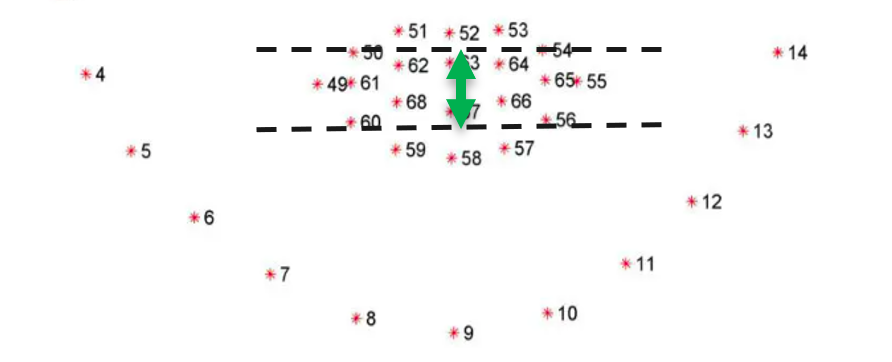
\includegraphics[width=0.7\textwidth]{Images/1_AI/yawn_distance.png}
    \caption{Facial landmarks for yawning detection.}
    \label{fig:yawn_distance}
\end{figure}

By measuring the distance between the upper and lower lip landmarks (Figure \ref{fig:yawn_distance}), the algorithm can determine if the mouth is open, which is a key indicator of yawning. A significant increase in this distance indicates a yawn, suggesting that the driver may be fatigued.

Yawning detection also relies on a threshold, often determined by the vertical distance between upper and lower lip landmarks. While specific thresholds can vary, values around \textcolor{red}{0.5 to 1.0} have been used experimentally. Adjusting this threshold helps in accurately identifying yawning events, crucial for assessing driver fatigue in monitoring systems, despite varying facial expressions and conditions.

By integrating these advanced detection methods, the driver monitoring system can effectively assess driver fatigue and drowsiness, contributing to improved road safety.
